\documentclass[letterpaper, 12pt]{article}
\usepackage{graphicx}
%This is the margin, it makes stuff look pretty but it's really not needed
\usepackage[margin=1in]{geometry}
%This package allows allows for headers and footers, which I think add to the look of the document
\usepackage{fancyhdr}

%The pagestyle calls from the fancyhdr package, but it can be set to a lot of other things without the package
\pagestyle{fancy}

%Gets rid of the default formatting when using the fancy pagestyle
\fancyhf{}
%Defining the header (by default, fancy includes a line on top and bot, I like it so I'm not getting rid of it!)
\rhead{
    Shengdong Li
    Calc 1
}
%Defining the footer
\rfoot{Page \thepage}

%The "body"/visible section of the tex file
\begin{document}
%Title page
\title{Response to Jyotsna Tera}
\author{by Shengdong Li}
\date{24 April 2020}
\maketitle

\section{Intro}
Hey Jyotsna! Great job on the comment to Alekhya, I really liked your visualization of the discs in the disc/washer method and concise explanations for your work. However, I noticed that you uploaded your work as a file in pdf format. Might I interest you in embedding to Canvas, to make your posts easier to read without downloading?
\section{Embedding a pdf to Canvas}
First, upload your pdf to Google Drive, and open it.
\begin{center}
    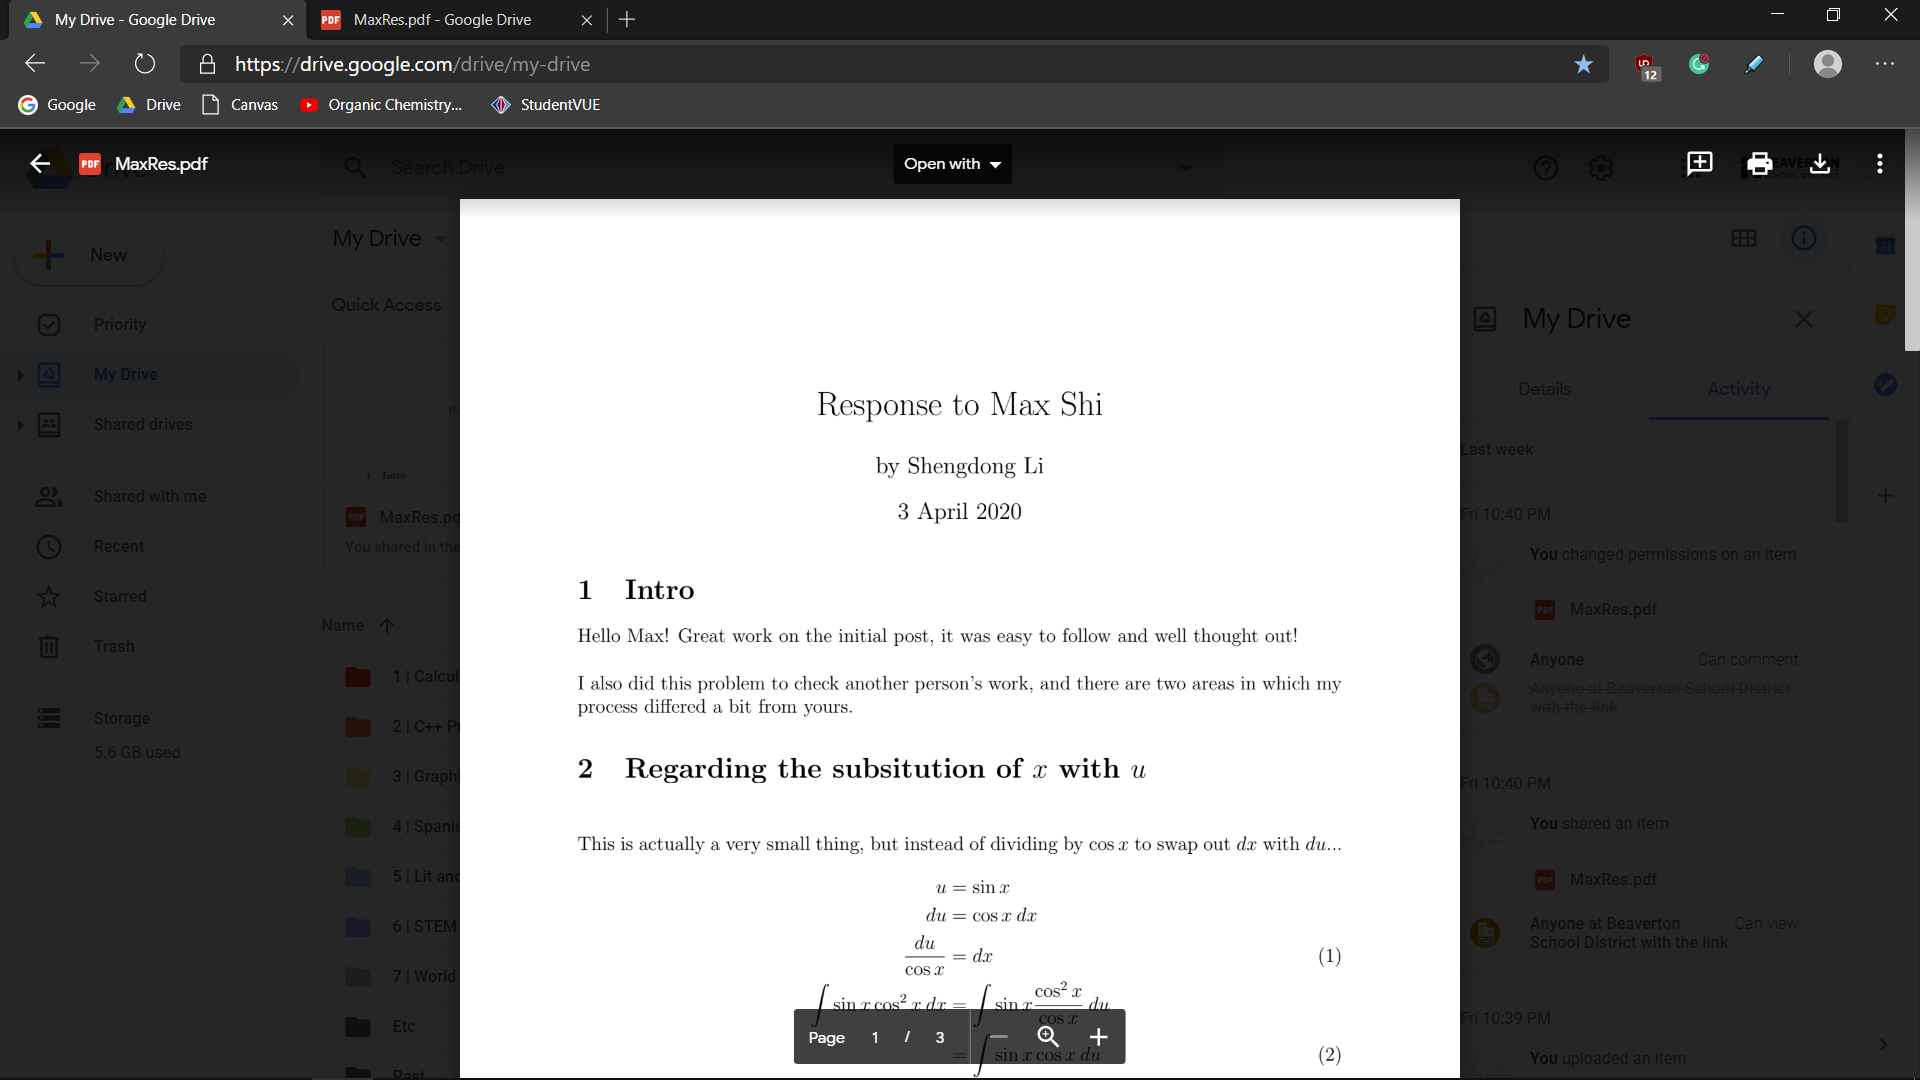
\includegraphics[scale=0.3]{1.png}
\end{center}
Then, change the sharing permissions on the document to something like "anyone at beaverton school district can find access" or other people will not be able to see your embedded file.
\begin{center}
    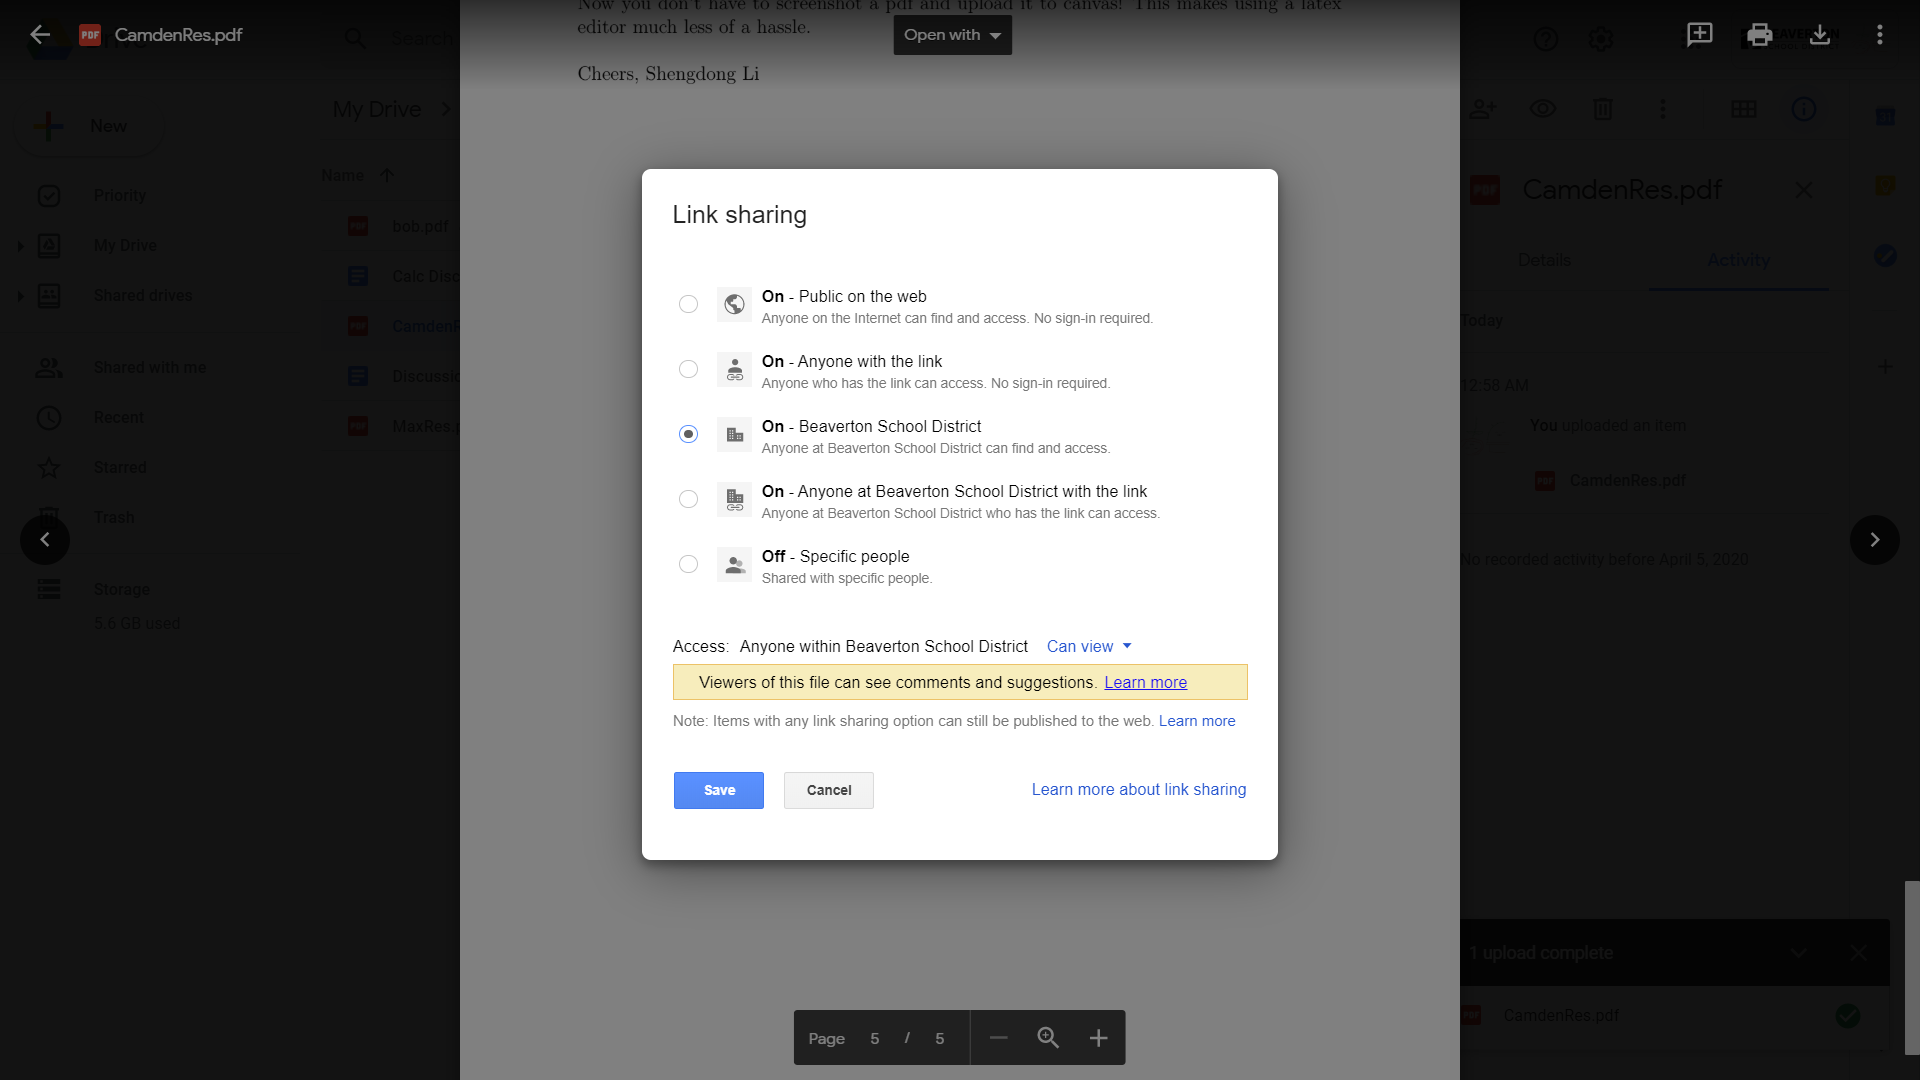
\includegraphics[scale=0.3]{9.png}
\end{center}
Then, click on the 3 dots on the top right, and click on open in new window
\begin{center}
    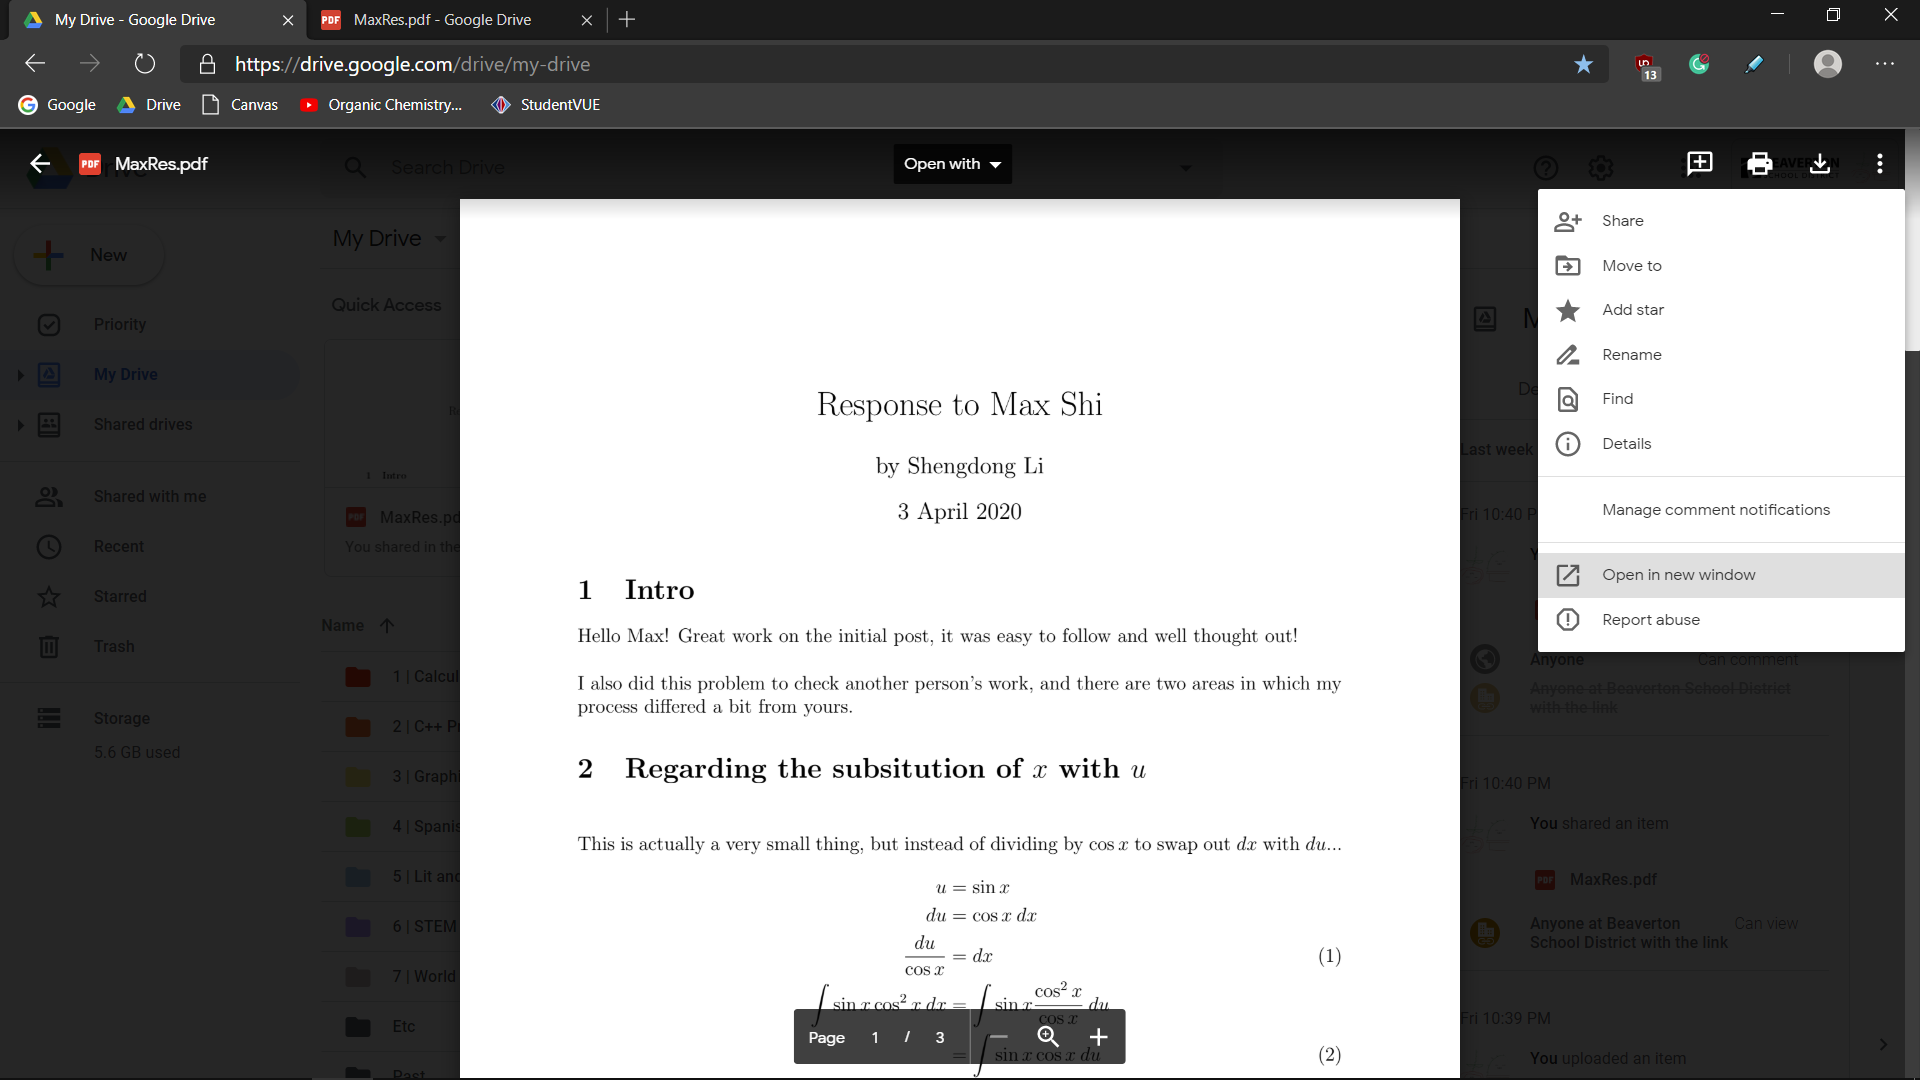
\includegraphics[scale=0.3]{2.png}
\end{center}
A new tab should pop up.
\begin{center}
    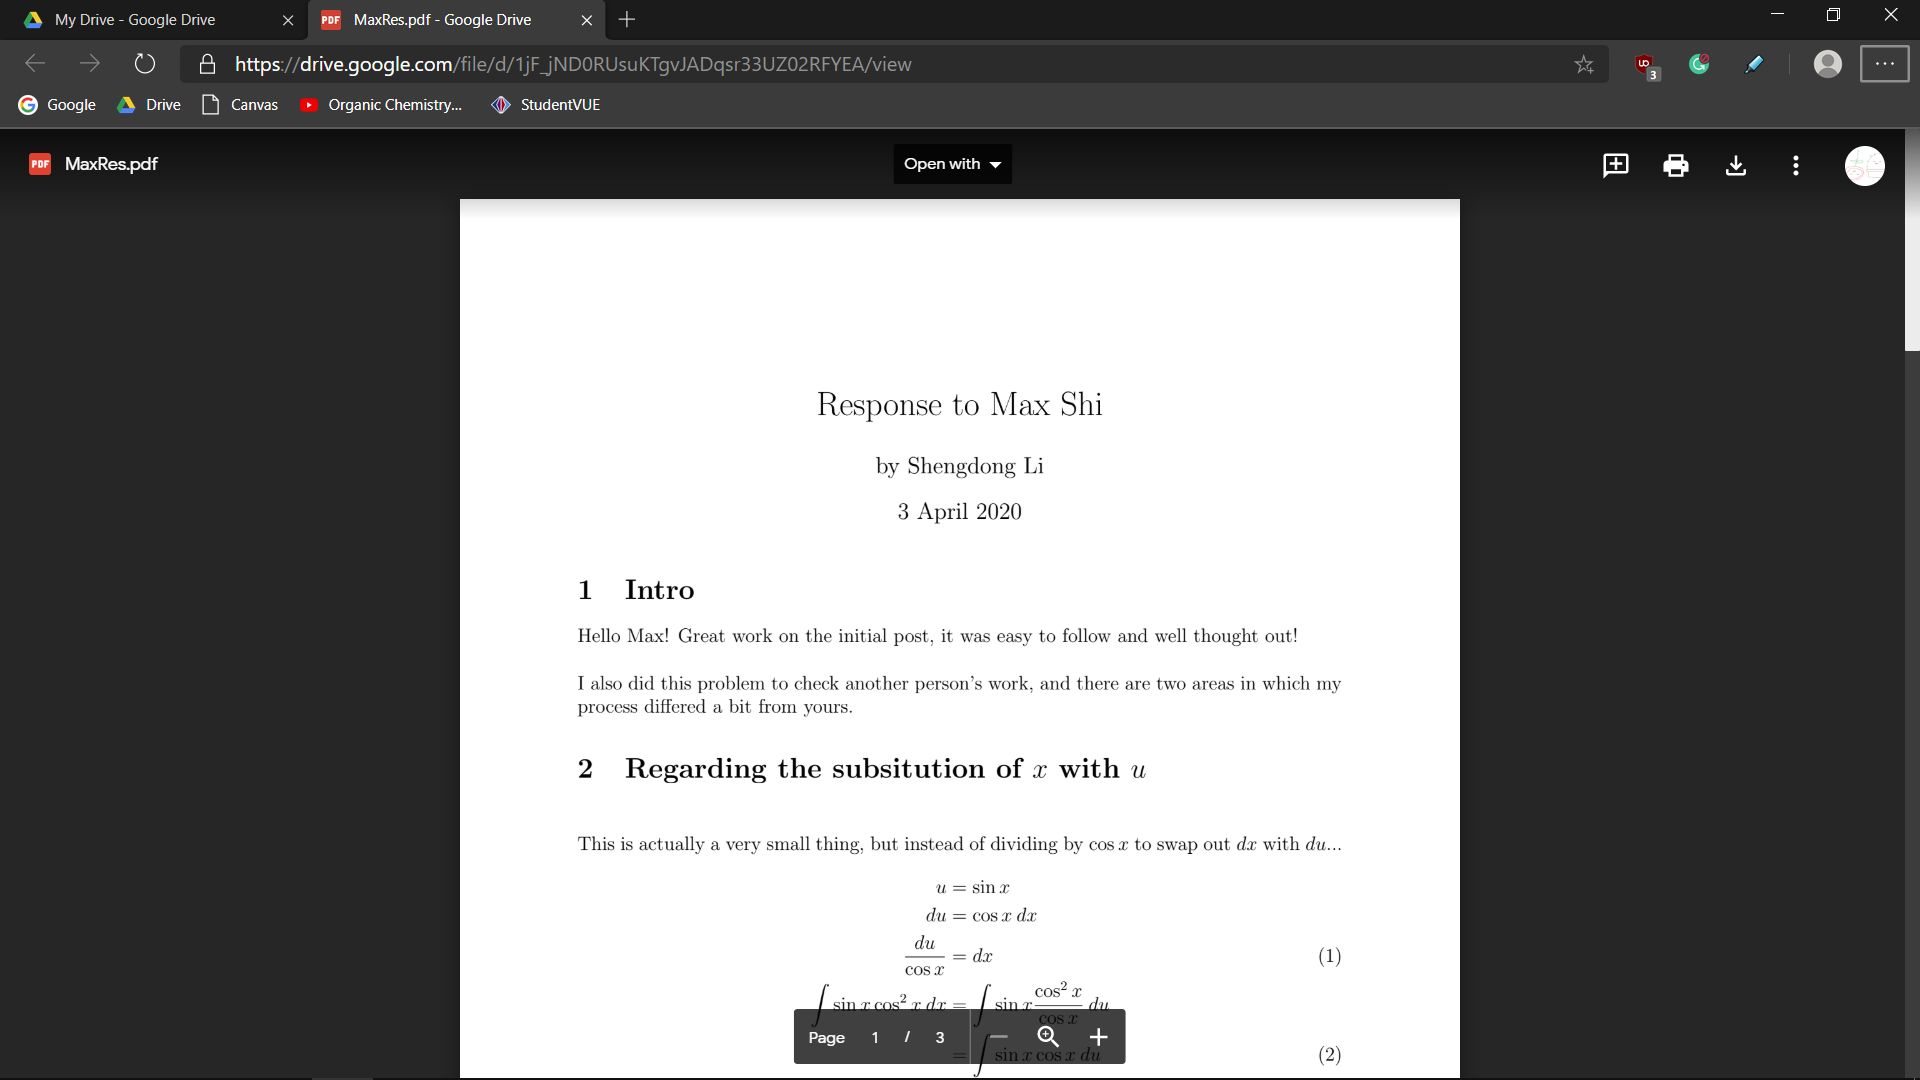
\includegraphics[scale=0.3]{3.png}
\end{center}
Click on the 3 dots on the top right again and then on embed item
\begin{center}
    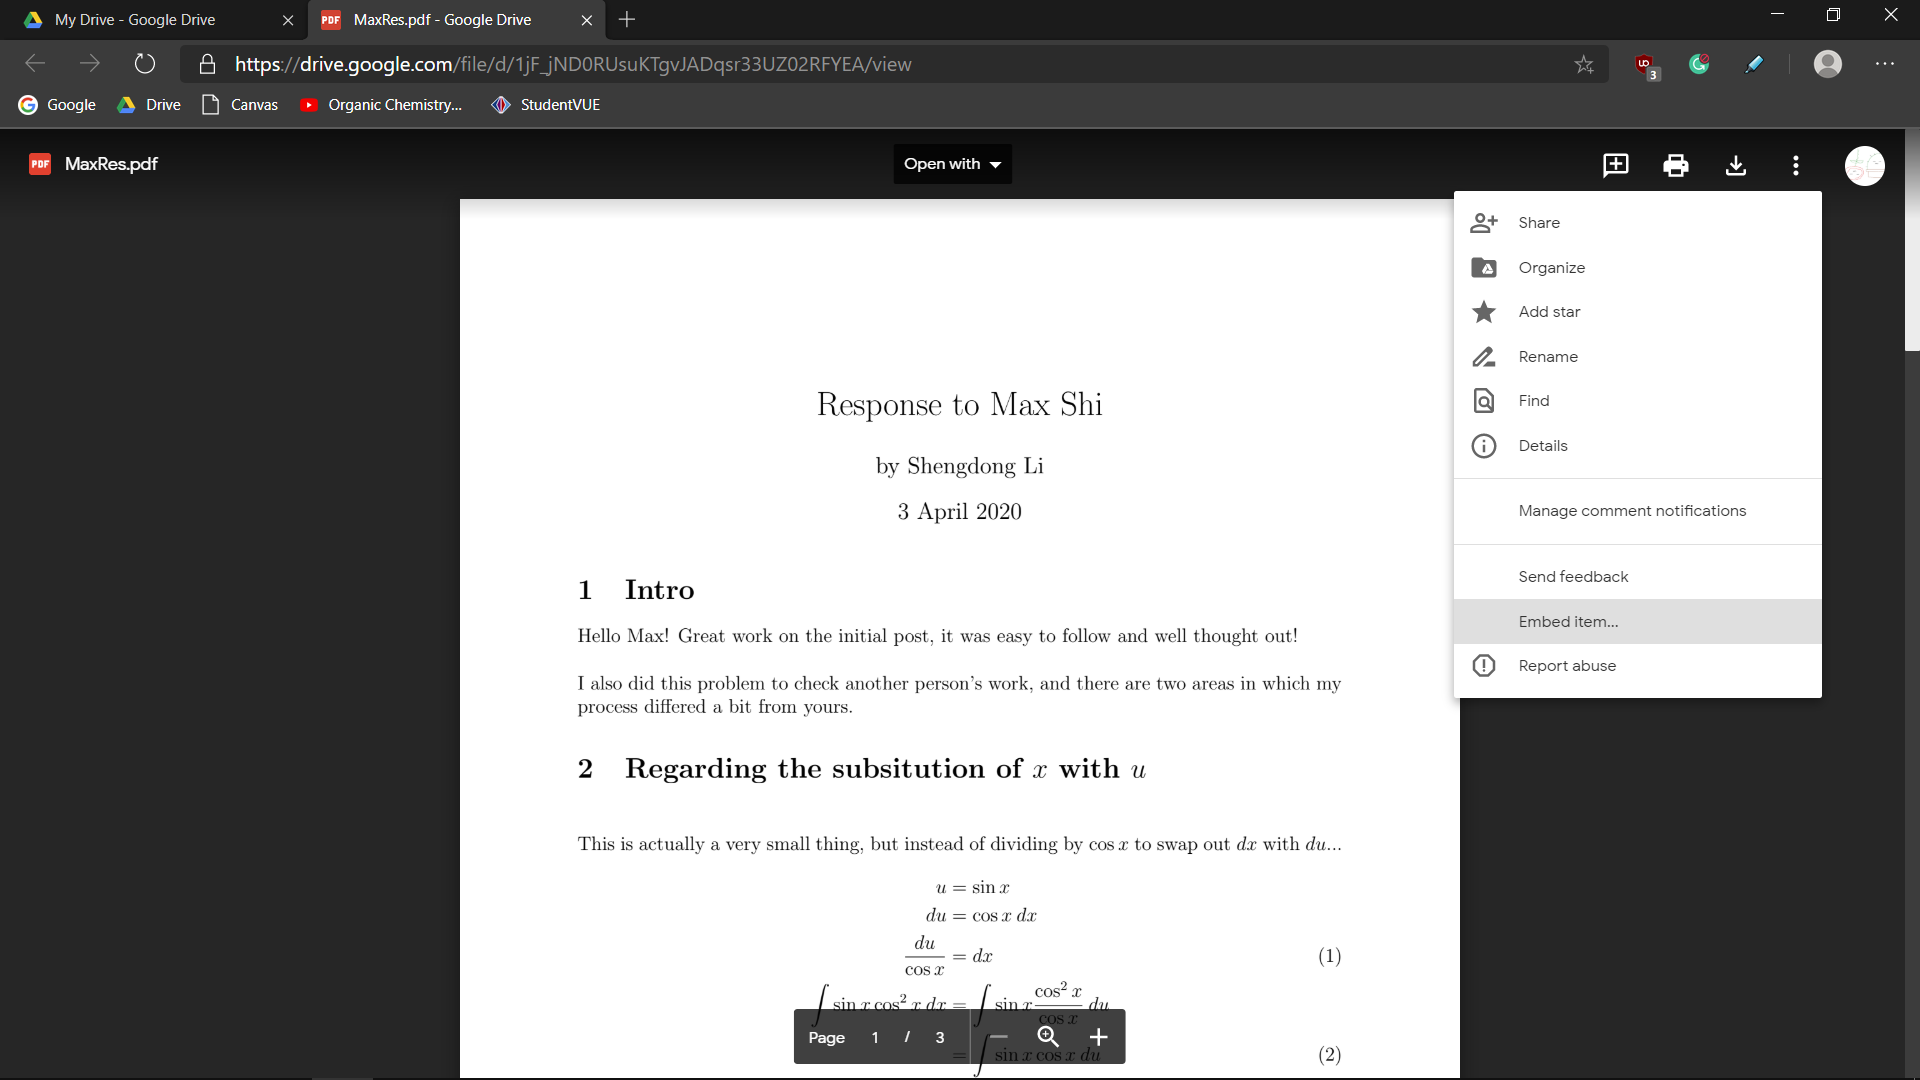
\includegraphics[scale=0.3]{4.png}
\end{center}
This box should pop up. Copy the text in there.
\begin{center}
    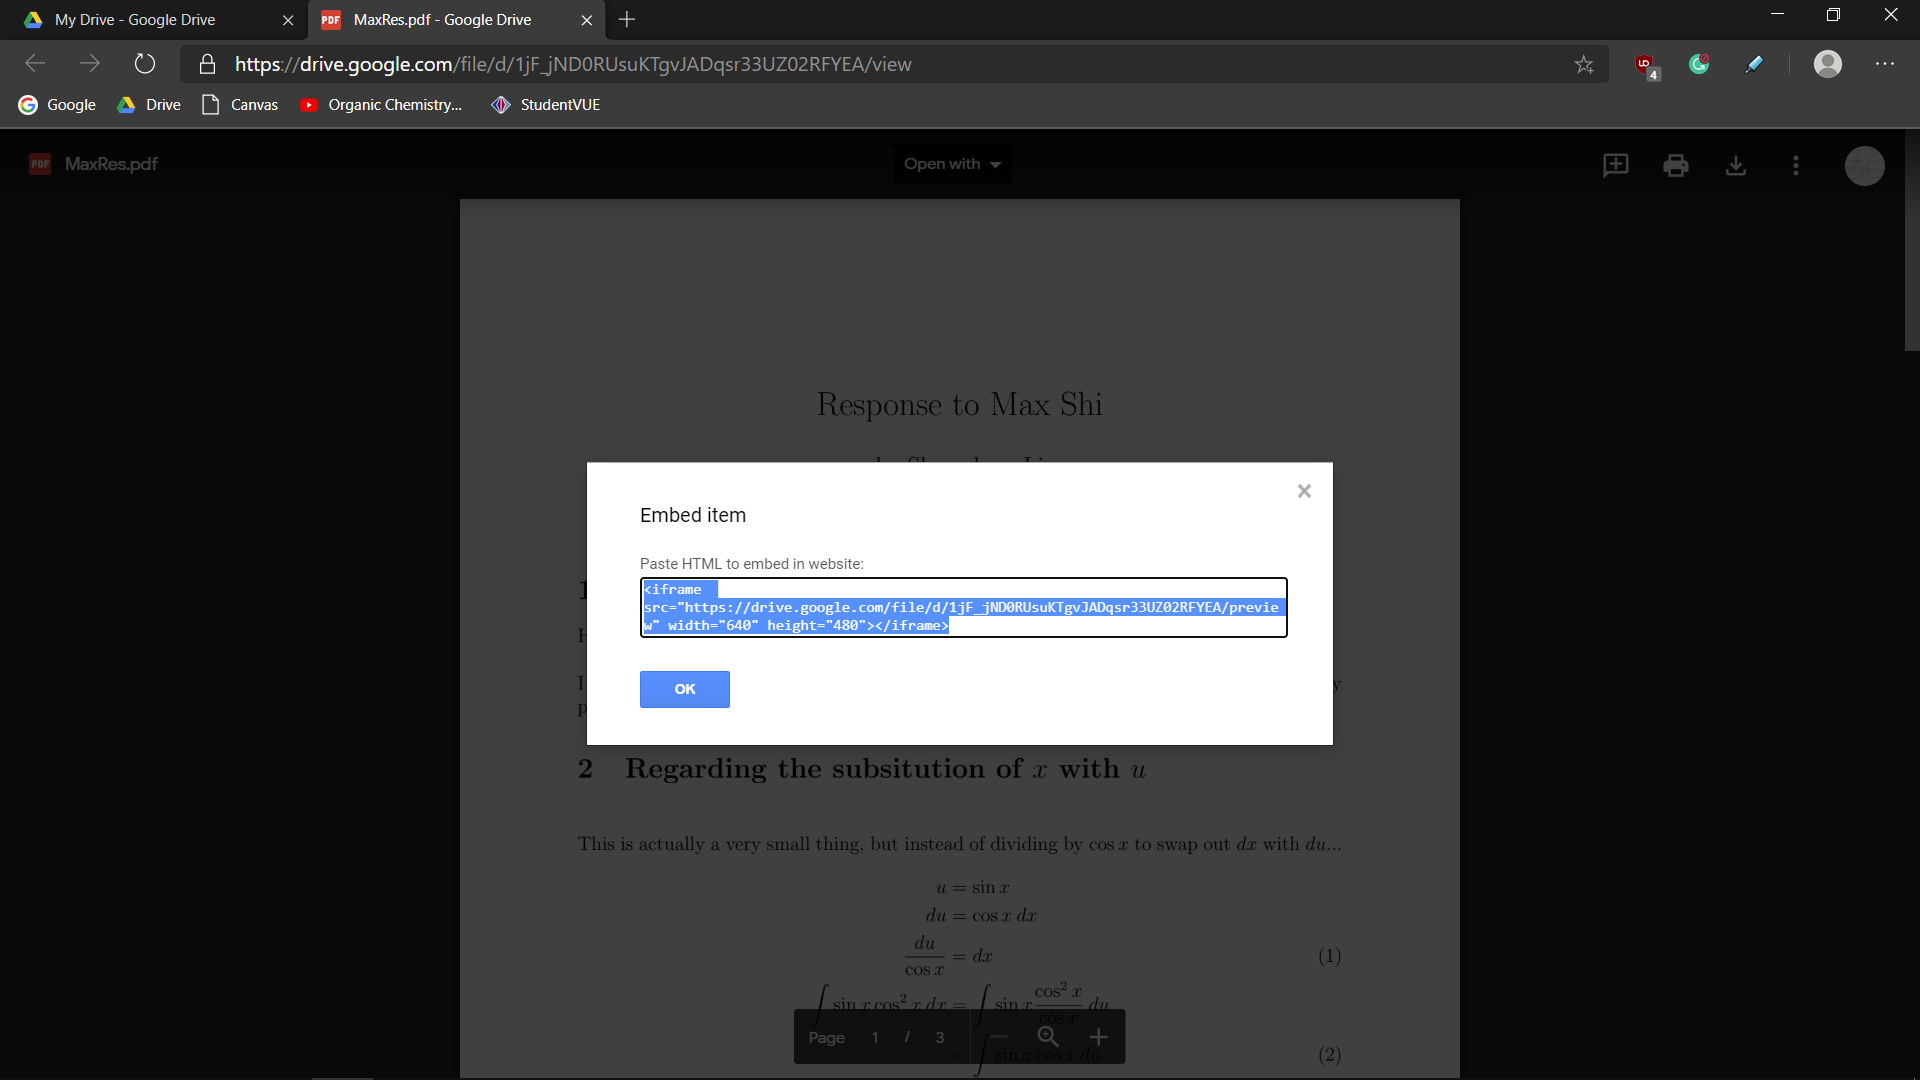
\includegraphics[scale=0.3]{5.png}
\end{center}
Then in Canvas, click on insert/edit media
\begin{center}
    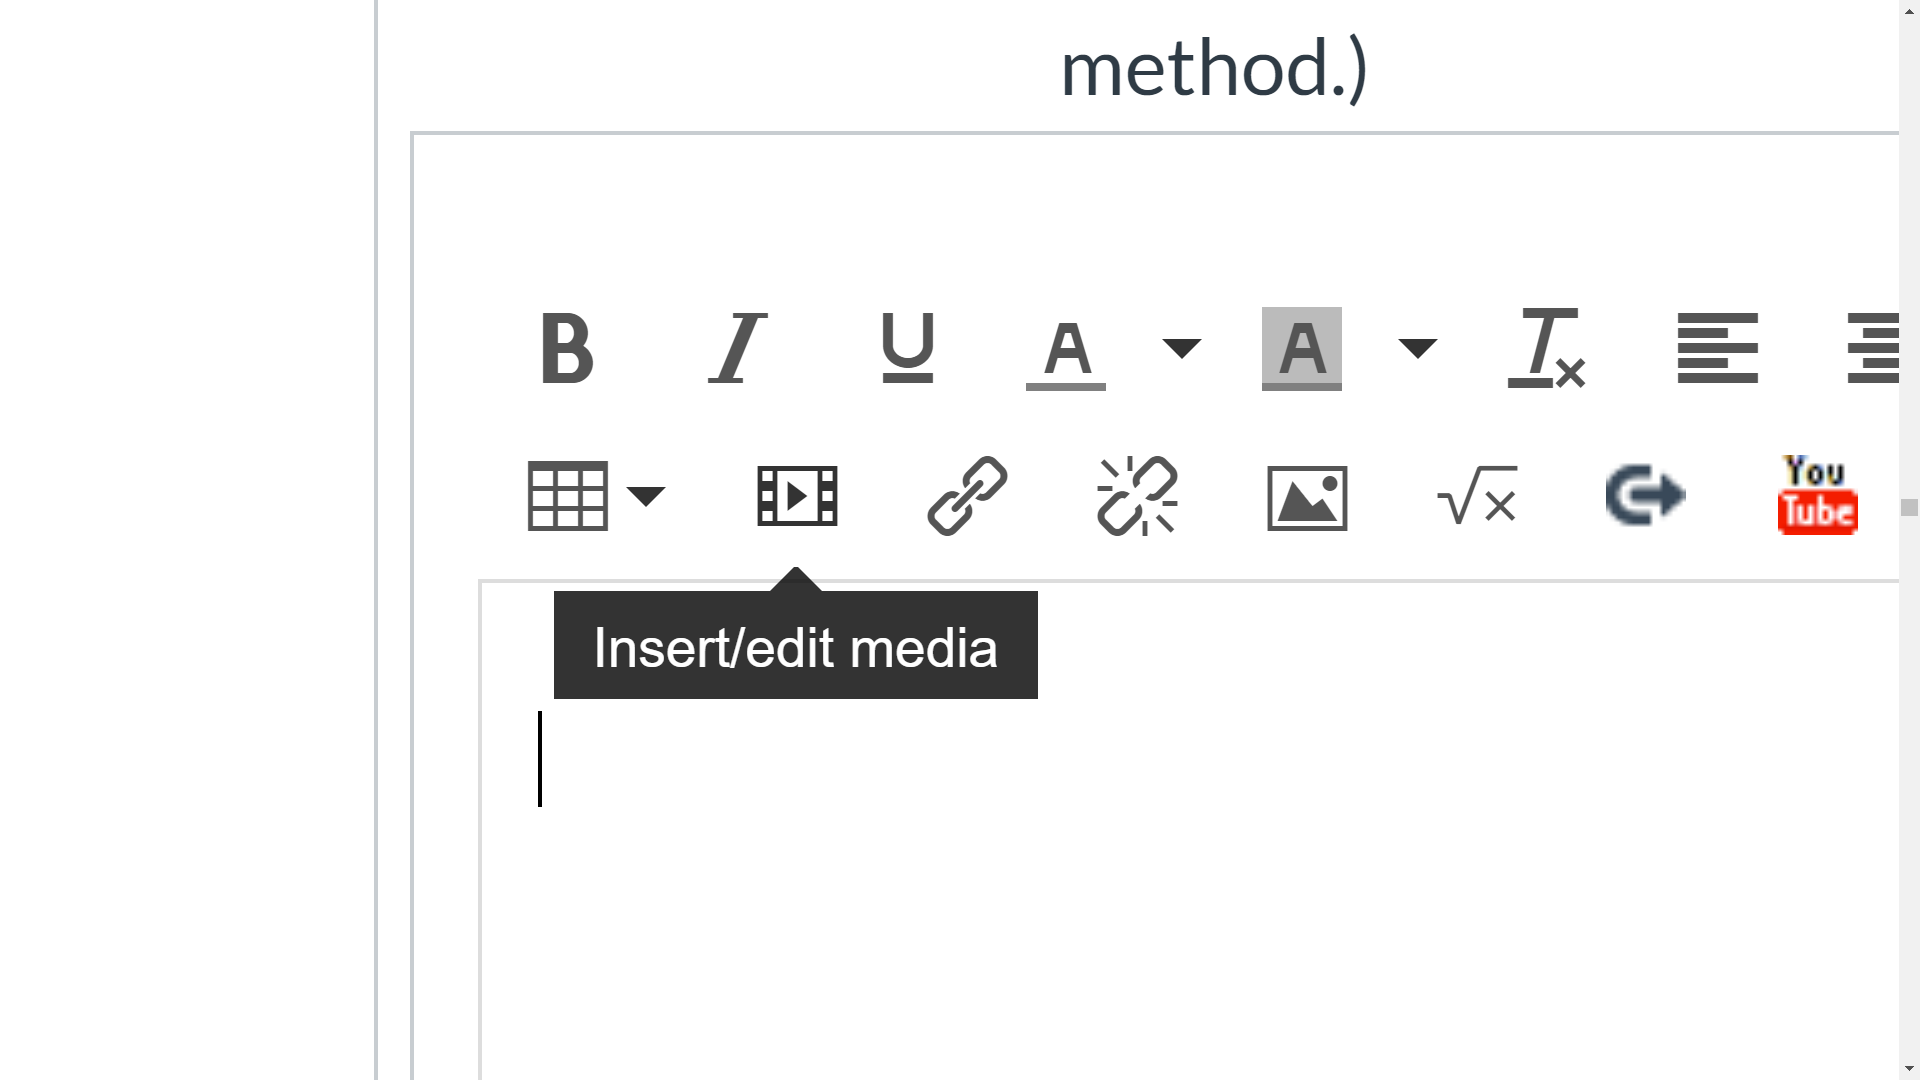
\includegraphics[scale=0.3]{6.png}
\end{center}
Open the embed tab, then copy and paste the embed code from earlier
\begin{center}
    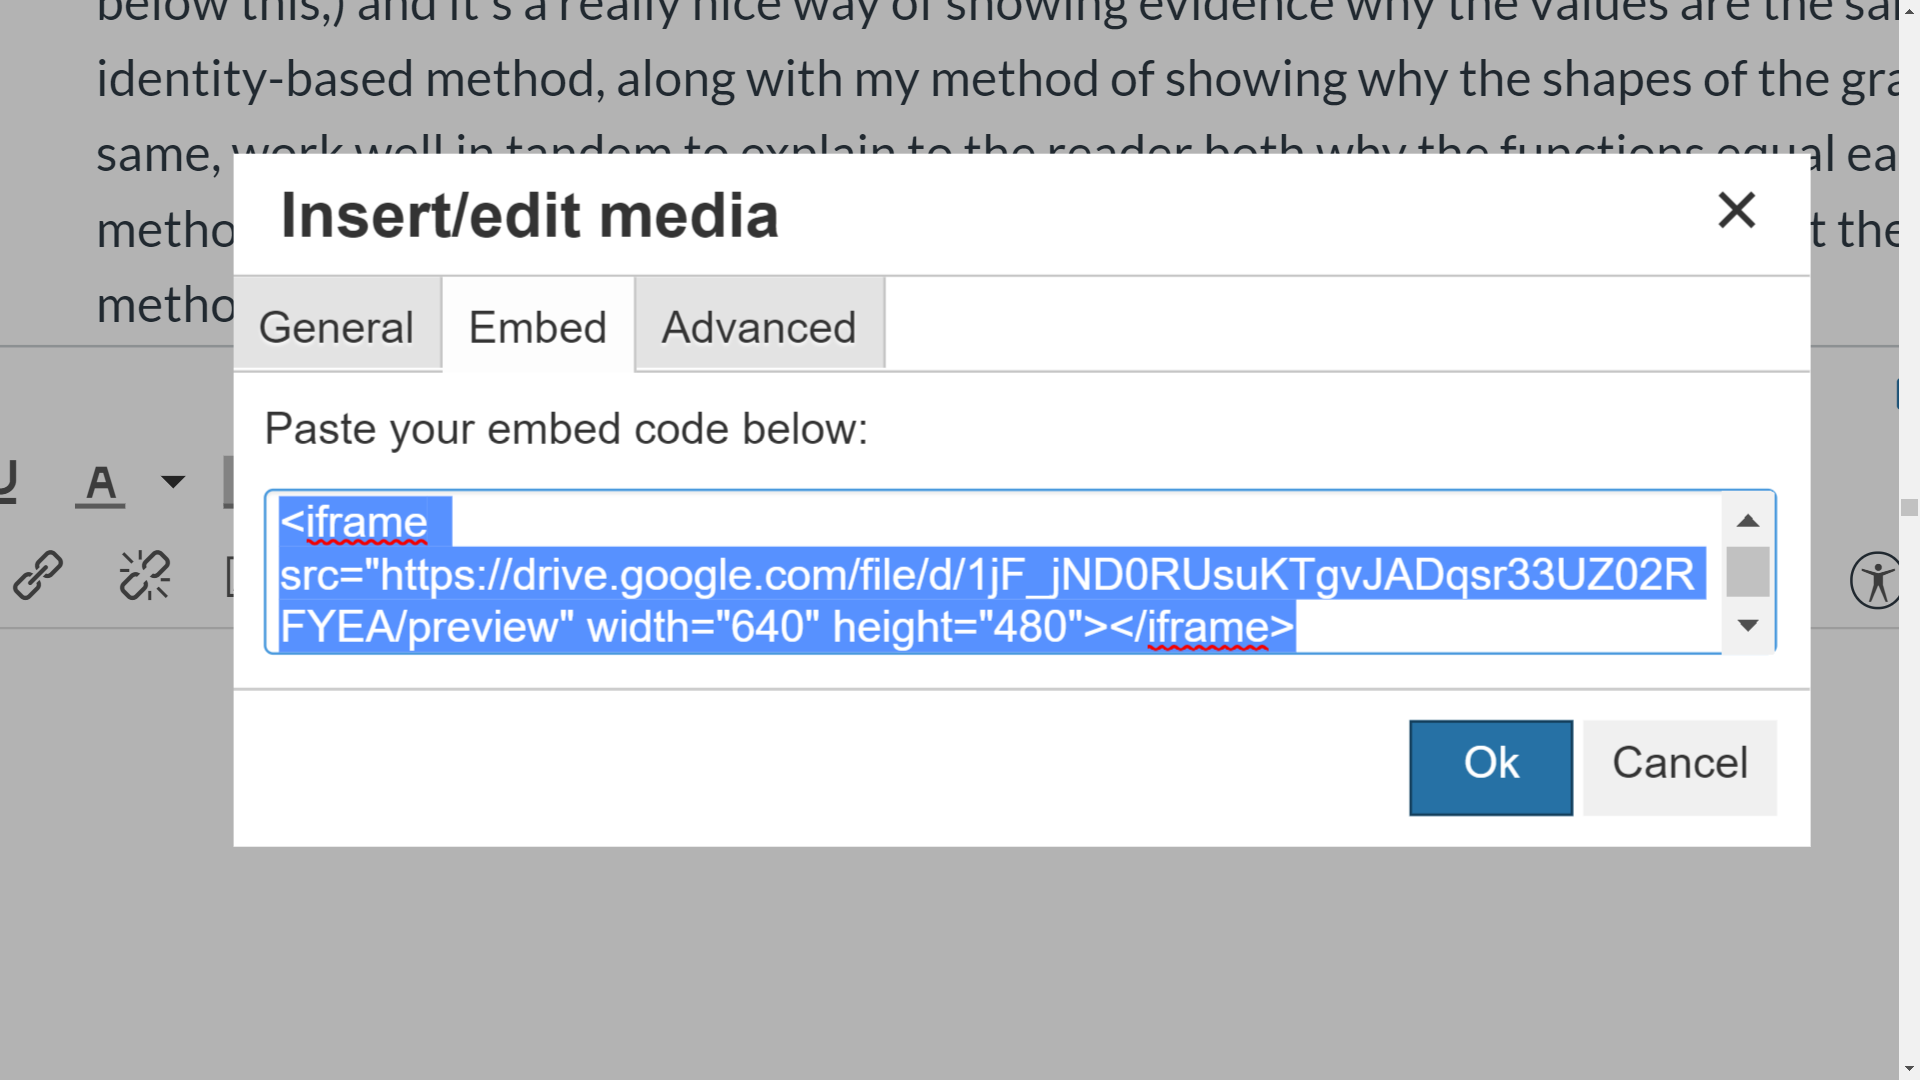
\includegraphics[scale=0.3]{7.png}
\end{center}
Click ok, and you should have an embedded item, like this:
\begin{center}
    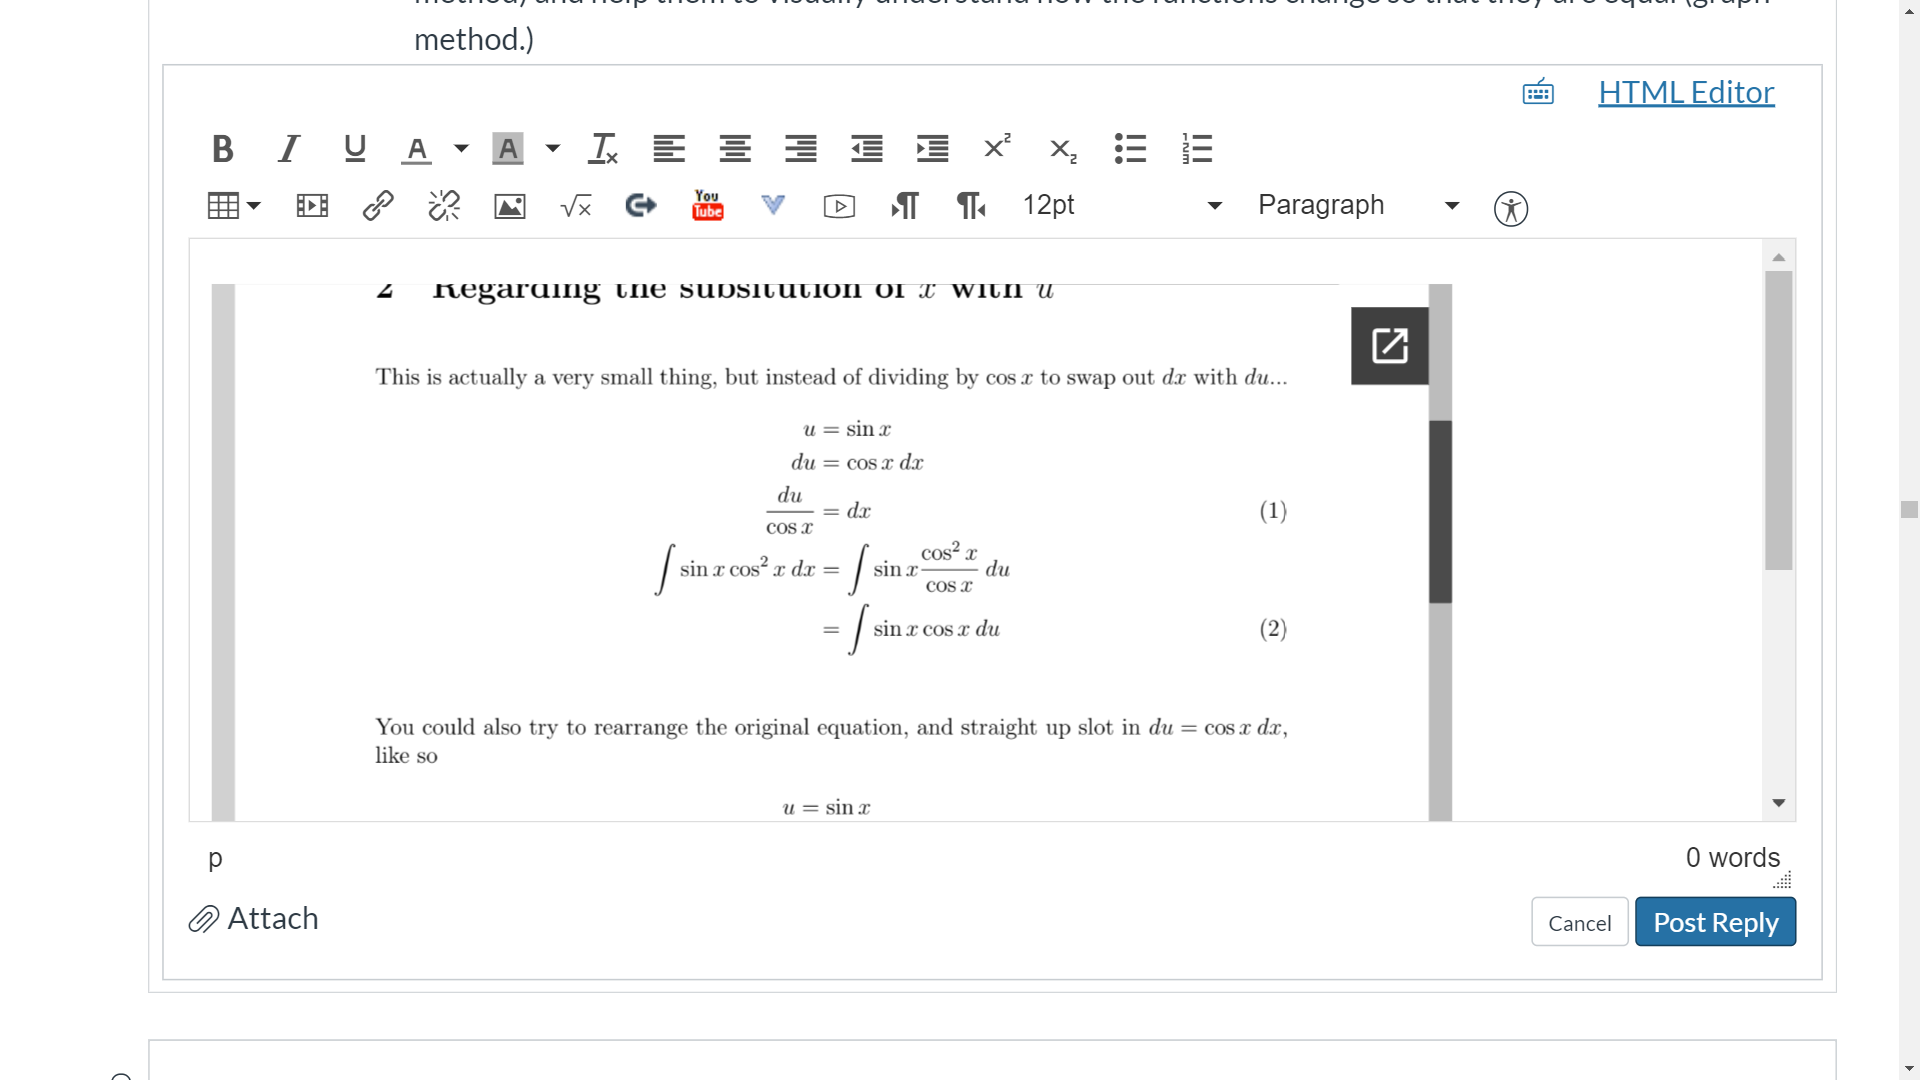
\includegraphics[scale=0.3]{8.png}
\end{center}
I hope that this helps! \bigbreak
Cheers, Shengdong Li
\end{document}